\documentclass[11pt,a4paper]{article}
\usepackage[utf8]{inputenc}
\usepackage[german]{babel}
\usepackage[T1]{fontenc}
\usepackage{amsmath}
\usepackage{amsfonts}
\usepackage{amssymb}
\usepackage{graphicx}
\usepackage[margin=1.25cm]{geometry} % Puts the same margin on all borders of the document

% Packages

\usepackage{hyperref} % Generate hyperlinks to referenced items
\usepackage{adjustbox} % Used to change parameters in \includegraphics[scale=•]{•}
\usepackage{enumitem} % Provides several options for lists
\usepackage{verbatim} % Package to use \begin{comment}
\usepackage{pdfpages} % Used to import PDF pages
\usepackage{multirow} % Allows us to have a single cell in a table span multiple rows
\usepackage{makecell} % Allows us to format multiple lines in a single cell
\usepackage{minted} % Used to syntax highlight code
\usepackage{xcolor}  % Gives access to coloring text
\usepackage{longtable} % Allows us to create a table over multiple pages
\usepackage{float} % Improved placement of floating items
\usepackage{pdfpages} % Used to import pdf pages
\usepackage{booktabs} % Used for horizontal lines instead of \hline



% Settings

\graphicspath{{./files/}} % Sets path for files to the files folder in the same directory

\hypersetup{
    colorlinks=false, %set true if you want colored links
    linktoc=all,     %set to all if you want both sections and subsections linked
    linkcolor=blue,  %choose some color if you want links to stand out
}

%\usepackage[none]{hyphenat} If I want to disable hyphenation

\begin{titlepage}
  \title{Mathematik II für Informatik - Zusammenfassung} % document_name-type_of_document
  \author{Jonas Milkovits}
  \date{Last Edited: \today}
\end{titlepage}

\setlist{nosep} % no space between list elements

\begin{document}

\pagenumbering{gobble}
\maketitle
\pagenumbering{roman} % i, ii, iii on beginning pages, that don't have content
\tableofcontents
\clearpage
\pagenumbering{arabic} % 1,2,3 on content pages

\begin{comment}
\noindent
\textbf{Definitionen}
\begin{table}[H]  
\begin{tabularx}{\textwidth}{X m{16cm}}
    \toprule
    
    & \\

    \bottomrule
    
\end{tabularx}
\end{table}

\noindent 
\textbf{Sätze}
\begin{table}[H]
\begin{tabularx}{\textwidth}{X m{16cm}}
    \toprule

    & \\

    \bottomrule
\end{tabularx}
\end{table}

\noindent
\textbf{Bemerkungen}
\begin{table}[H]
\begin{tabularx}{\textwidth}{X m{16cm}}
    \toprule

    & \\

    \bottomrule
\end{tabularx}
\end{table}

\noindent
\textbf{Beispiele}
\begin{table}[h]
\begin{tabularx}{\textwidth}{X m{16cm}}
    \toprule

    & \\

    \bottomrule
\end{tabularx}
\end{table}
\end{comment}

\section{Analysis Teil I - Konvergenz und Stetigkeit}
\subsection{Die reellen Zahlen}
\noindent
\textbf{Definitionen} 
\begin{table}[H]  
\begin{tabularx}{\textwidth}{X m{16cm}}
    \toprule
    
    5.1.1 & Die \textbf{Menge der reellen Zahlen} ist der kleinste angeordnete Körper, 
            der $\mathbb{Z}$ enthält und das Vollständigskeitsaxiom 
            \textit{"Jede nichtleere Teilmenge, die eine obere Schranke besitzt, hat ein Suprenum."}
            erfüllt. \\
    \midrule
    5.1.3 & Eine Teilmenge $M \subseteq \mathbb{R}$ heißt:
            \begin{itemize}[topsep=-0.5cm]
                \item[a)] nach \textbf{oben (unten) beschränkt}, wenn sie eine obere (untere) Schranke besitzt.
                \item[b)] \textbf{beschränkt}, wenn sie nach oben und unten beschränkt ist. 
            \end{itemize} \vspace{-0cm} \\
    \midrule
    5.1.5 & Die Funktion $|\cdot|: \mathbb{R} \rightarrow \mathbb{R}$ mit \hfill \break
            \centerline{    
                $|x| =  \begin{cases}
                x & \text{falls x $\geq$ 0} \\
                -x & \text{falls x < 0}
               \end{cases}$
            } \hfill \break
            heißt \textbf{Betragsfunktion} und $|x|$ heißt Betrag von $x$. \\
    \midrule
    5.1.8 & \textbf{Intervalle:} \hfill \break 
            Es seien zwei Zahlen $a,b \in \mathbb{R}$ mit $a < b$ gegeben. Dann heißen:
            \begin{itemize}[topsep=-0.5cm]
                \item $(a,b):= \{x \in \mathbb{R}: a < x < b\}$ offenes Intervall
                \item $[a,b]:= \{x \in \mathbb{R}: a \leq x \leq b\}$ abgeschlossenes Intervall
                \item $(a,b]:= \{x \in \mathbb{R}: a < x \leq b\}$ halboffenes Intervall
                \item $[a,b):= \{x \in \mathbb{R}: a \leq x < b\}$ halboffenes Intervall
            \end{itemize} \vspace{-0cm} \hfill \break
            \textbf{Halbstrahlen:}
            \begin{itemize}[topsep=-0.5cm]
                \item $[a,\infty) := \{x \in \mathbb{R} : a \leq x\}$
                \item $(a, \infty) := \{x \in \mathbb{R} : a < x\}$
                \item $(-\infty, a] := \{x \in \mathbb{R}: x \leq a\}$
                \item $(-\infty,a) := \{x \in \mathbb{R} : x < a\}$
                \item $(-\infty,\infty):= \mathbb{R}$
            \end{itemize} \vspace{-0cm} \\
    \bottomrule
    
\end{tabularx}
\end{table}

\noindent
\textbf{Sätze}
\begin{table}[H]
\begin{tabularx}{\textwidth}{X m{16cm}}
    \toprule

    5.1.4 & Jede nach unten beschränkte, nichtleere Teilmenge von $\mathbb{R}$ besitzt ein Infimum. \linebreak
            (Umkehrung Vollständigkeitsaxiom) \\
    \midrule
    5.1.6 & \textbf{Rechenregeln Betragsfunktion:} \hfill \break
            Für alle $x,y \in \mathbb{R}$ gilt: 
            \begin{itemize}[topsep=-0.5cm]
                \item[a)] $|x| \geq 0$
                \item[b)] $|x| = |-x|$
                \item[c)] $\pm x \leq |x|$
                \item[d)] $|xy| = |x| \cdot |y|$
                \item[e)] $|x| = 0$ genau dann, wenn $x = 0$
                \item[f)] $|x+y| \leq |x| + |y|$ (Dreiecksungleichung)  
            \end{itemize} \vspace{-0cm} \\

    

    \bottomrule
\end{tabularx}
\end{table}

\noindent
\textbf{Bemerkungen}
\begin{table}[H]
\begin{tabularx}{\textwidth}{X m{16cm}}
    \toprule

        &   Ein Körper mit Totalordnung $\leq$ heißt \textbf{angeordneter Körper}, falls gilt:
            \begin{itemize}[topsep=-0.5cm]
                \item $\forall a,b,c \in K: a \leq b \Rightarrow a + c \leq b + c$
                \item $\forall a,b,c \in K: (a \leq b$ und $0 \leq c) \Rightarrow ac \leq bc$
            \end{itemize} \vspace{-0cm} \\

    \bottomrule
\end{tabularx}
\end{table}

\pagebreak

\subsection{Wurzeln, Fakultäten und Binomialkoeffizienten}
\noindent
\textbf{Definitionen}
\begin{table}[H]  
\begin{tabularx}{\textwidth}{X m{16cm}}
    \toprule
    
    5.2.1 & \textbf{Ganzzahlige Potenzen:} \hfill \break
            Für jedes $x\in \mathbb{R}$ und jedes $n \in \mathbb{N^*}$ ist
            \begin{itemize}[topsep=-0.5cm]
                \item[a)] $x^n := x \cdot x \cdot x ... \cdot x$ ($n$-mal $x$)
                \item[b)] $x^{-n} := \frac{1}{x^n}$, falls $x\neq 0$
                \item[c)] $x^0 := 1$  
            \end{itemize} \vspace{-0cm} \\
    \midrule
    5.2.3 & Es seien $a \in \mathbb{R_+}$ und $n \in \mathbb{N^*}$. Die \textbf{eindeutige Zahl} $x^n \in \mathbb{R_+}$ mit 
            $x^n = a$ heißt $n$-te \textbf{Wurzel} von $a$ und man schreibt $x = \sqrt[n]{a}$. Für den wichtigsten Fall $n = 2$ 
            gibt es die Konvention $\sqrt{a} := \sqrt[2]{a}$. \\
    \midrule
    5.2.5 & Aus der Eindeutigkeit der $n$-ten Wurzel (5.2.4) folgt: \hfill \break
            Für jedes $x \in \mathbb{R_+}$ und jedes $q = \frac{n}{m} \in \mathbb{Q}$ mit $n \in \mathbb{Z}$ und 
            $m \in \mathbb{N^*}$ ist die \textbf{rationale Potenz} definiert durch: \hfill \break
            \centerline{$x^q = x^{\frac{n}{m}} := (\sqrt[x]{x})^n$.} \\
    \midrule
    5.2.7 & Es sei $n \in \mathbb{N^*}$. Dann wird die Zahl $n! := 1 \cdot 2 \cdot ... \cdot n$ als $n$ \textbf{Fakultät} bezeichnet. \hfill \break
            Weiterhin definieren wir $0! := 1$. \hfill \break
            Es seien $n,k \in \mathbb{N}$ mit $k \leq n$. Dann heißt $\binom{n}{k} := \frac{n!}{k!(n-k)!}$ \textbf{Binomialkoeffizient} 
            \string"$n$ über $k$\string". \\
    \bottomrule
    
\end{tabularx}
\end{table}

\noindent
\textbf{Sätze}
\begin{table}[H]
\begin{tabularx}{\textwidth}{X m{16cm}}
    \toprule

    5.2.2 & \textbf{Existenz der Wurzel:} \hfill \break 
            Für jedes $a \in R_+$ und alle $n \in N^*$ gibt es genau ein $w \in R_+$ mit $x^n = a$. \\
    \midrule
    5.2.4 & Es seien $q \in \mathbb{Q}$ und $m,ü \in \mathbb{Z}$, sowie $n,r \in \mathbb{N^*}$ so, dass
            $q = \frac{m}{n} = \frac{p}{r}$. \hfill \break
            Dann gilt für jedes $x \in \mathbb{R_+}$: $(\sqrt[n]{x})^m = (\sqrt[r]{m})^p$. \\
    \midrule
    5.2.9 & Es seien $n,k \in \mathbb{N}$ mit $k \leq n$ und $a,b \in \mathbb{R}$. Dann gilt:
            \begin{itemize}[topsep=-0.5cm]
                \item[a)] $\binom{n}{0} = \binom{n}{n} = 1$ und $\binom{n}{k} + \binom{n}{k-1} = \binom{n+1}{k}$
                \item[b)] $a^{n+1} - b^{n+1} = (a-b) \sum^n_{k=0}a^{n-k}b^k$
                \item[c)] $(a+b)^n = \sum^n_{k=0} \binom{n}{k} a^{n-k}b^k$ (Binomialformel)  
            \end{itemize} \vspace{-0cm} \\
    

    \bottomrule
\end{tabularx}
\end{table}

\noindent
\textbf{Bemerkungen}
\begin{table}[H]
\begin{tabularx}{\textwidth}{X m{16cm}}
    \toprule

    5.2.6 & \textbf{Rechenregeln für Potenzen (auch rational)} \hfill \break
            $\forall x,y \in \mathbb{R_+} \textbackslash \{0\}$ und $\forall p,q \in \mathbb{Q}$ gilt: 
            \begin{itemize}[topsep=-0.5cm]
                \item $x^p x^q = x^{p+q}$
                \item $x^py^p = (xy)^p$
                \item $(x^p)^q = x^{pq}$
                \item $\frac{x^p}{x^q} = x^{p-q}$
                \item $\frac{x^p}{y^p} = (\frac{x}{y})^p$
            \end{itemize} \vspace{-0cm} \\
    \midrule
    5.2.8 & \textbf{Fakultät und Binomialkoeffizient} \hfill \break
            $n!$ ist die Anzahl der möglichen Reihenfolgen von $n$ unterschiedlichen Dingen. \hfill \break
            $\binom{n}{k}$ ist die Anzahl der Möglichkeiten aus $n$ unterscheidbaren Dingen genau $k$ auszuwählen. \\
    \midrule
          & Zugriff auf \textbf{Binomialkoeffizienten} für binomische Formeln durch Pascal'sches Dreieck \\
    \bottomrule
\end{tabularx}
\end{table}

\subsection{Konvergenz von Folgen}
\subsubsection{Der Konvergenzbegriff und wichtige Beispiele}

\noindent
\textbf{Definitionen}
\begin{table}[H]  
\begin{tabularx}{\textwidth}{X m{16cm}}
    \toprule
    
    5.3.1 & Es sei $(a_n)$ eine Folge in $\mathbb{K}$ und $a \in \mathbb{K}$. Die Folge $(a_n)$ heißt \textbf{konvergent} gegen $a$,
            falls für jedes $\epsilon > 0$ ein $n_0 \in \mathbb{N}$ exisitert mit \hfill \break
            \centerline{$|a_n-a| < \epsilon$ für alle $n \geq n_0$.}
            In diesem Fall heißt $a$ der \textbf{Grenzwert} oder Limes von $(a_n)$ und wir schreiben: \hfill \break
            \centerline{$lim_{a \rightarrow \infty} = a$ oder $a_n \rightarrow a (n \rightarrow \infty)$.} 
            Ist $(a_n)$ eine Folge $\mathbb{K}$, die gegen kein $a \in \mathbb{K}$ konvergiert, so heißt diese \textbf{divergent}. \\
    \midrule
    5.3.4 & Eine Folge $(a_n)$ in $\mathbb{K}$ heißt \textbf{beschränkt}, wenn die Menge $\{a_n: n \in \mathbb{N}\} = \{a_0,a_1,a_2,...\}$
            beschränkt in $\mathbb{K}$ ist. \hfill \break
            Ist $\mathbb{K} = \mathbb{R}$, so setzen wir weiter \hfill \break
            \centerline{$sup_{n \in \mathbb{N}}a_n := sup^{\infty}_{n=0}a_n := sup\{a_n: n \in \mathbb{N}\}$} 
            \centerline{$inf_{n \in \mathbb{N}}a_n := inf^{\infty}_{n=0}a_n := inf\{a_n: n \in \mathbb{N}\}$} \\
    \midrule
    5.3.13& \textbf{Bestimmte Divergenz:} \hfill \break
            Eine Folge $(a_n)$ in $\mathbb{R}$ \textbf{divergiert bestimmt nach $\infty (- \infty)$} und wir schreiben
            $lim_{n \rightarrow \infty} a_n = \infty (-\infty)$, wenn es für jedes $C \geq 0$ ein $n_0 \in \mathbb{N}$ gibt, so dass
            $a_n \geq C (a_n \leq -C)$ für alle $n \leq n_0$ gilt. \\


    \bottomrule
    
\end{tabularx}
\end{table}

\noindent 
\textbf{Sätze}
\begin{table}[H]
\begin{tabularx}{\textwidth}{X m{16cm}}
    \toprule

    5.3.5 & Jede \textbf{konvergente Folge} in $\mathbb{K}$ ist \textbf{beschränkt}. \hfill \break
            Die Umkehrung dieses Satzes ist \textbf{falsch}. Es gibt beschränkte Folgen, die nicht konvergieren. \\
    \midrule
    5.3.7 & \textbf{Grenzwertsätze} \hfill \break
            Es seien $(a_n), (b_n)$ und $(c_n)$ Folgen in $\mathbb{K}$. Dann gilt:
            \begin{itemize}
                \item[a)] Ist $lim_{n\rightarrow \infty} a_n = a$, so gilt $lim_{n \rightarrow \infty} |a_n| = |a|$
                \item[b)] Gilt $lim_{n \rightarrow \infty} a_n = a$ und $lim_{n \rightarrow \infty} b_n = b$ so gilt:
                    \begin{itemize}
                        \item[i)] $lim_{n \rightarrow \infty}(a_n + b_n) = a + b$
                        \item[ii)] $lim_{n \rightarrow \infty} (a_n \cdot b_n) = a \cdot b$
                        \item[iii)] $lim_{n \rightarrow \infty} (\alpha a_n) = \alpha a$ für alle $\alpha \in \mathbb{K}$
                        \item[iv)] Ist zusätzlich $b_n \neq 0$ für alle $n \in \mathbb{N}$ und $b \neq 0$, 
                                    so ist $lim_{n \rightarrow \infty} \frac{a_n}{b_n} = \frac{a}{b}$
                    \end{itemize} 
            \end{itemize}
            Ist $\mathbb{K} = \mathbb{R}$, so gilt außerdem:
            \begin{itemize}[topsep=-0.5cm]
                \item[c)] Ist $a_n \leq b_n$ für alle $n \in \mathbb{N}$ und $lim_{n \rightarrow \infty} a_n = a$ sowie 
                            $lim_{n \rightarrow \infty} b_n = b$, so folgt $a \leq b$
                \item[d)] Ist $a_n \leq c_n \leq b_n$ für alle $n \in \mathbb{N}$ und sind $(a_n)$ und $(b_n)$ konvergent mit
                            $lim_{n \rightarrow \infty} a_n = lim_{n \rightarrow \infty} b_n = a$, so ist auf die Folge $(c_n)$
                            konvergent und es gilt $lim_{n \rightarrow \infty} c_n = a$ \hfill \break
                            \textbf{(Sandwich-Theorem)} 
            \end{itemize} \vspace{-0cm} \\


    \bottomrule
\end{tabularx}
\end{table}

\noindent
\textbf{Bemerkungen}
\begin{table}[H]
\begin{tabularx}{\textwidth}{X m{16cm}}
    \toprule

          & Sei $X$ eine Menge. Eine \textbf{Folge} in $X$ ist eine Abbildung $a: \mathbb{N} \rightarrow X$. \hfill \break
            (Für $X = \mathbb{R}$ reelle Folge, $X = \mathbb{C}$ komplexe Folge) \hfill \break
            Schreibweise: $a_n$ statt $a(n)$. ($n$-tes Folgeglied) \hfill \break
            Ganze Folge: $(a_n)_{n \in \mathbb{N}}$ oder $(a_n)$ oder $(a_n)_{n>0}$ \\
    \midrule
          & Folgen haben maximal einen (eindeutiger) Grenzwert \\
    \midrule
          & Bezeichnung von Folgen, für die der Grenzwert 0 ist: \textbf{\string"Nullfolge\string"} \\
    \midrule
    5.3.7 & c) ist falsch mit $<$, nur richtig mit $\leq$ \\
    \midrule
    5.3.10& \textbf{Wichtige konvergente Folgen}
            \begin{itemize}[topsep=-0.5cm]
                \item[a)] Ist $(a_n)$ eine konvergente Folge in $\mathbb{R}$ mit Grenzwert $a$ und gilt $a \geq 0$ für alle $n \in \mathbb{N}$
                            so ist für jedes $p \in \mathbb{N^*}$ auch $lim_{n \rightarrow \infty} \sqrt[p]{a_n} = \sqrt[p]{a}$.
                \item[b)] Die Folge $(q^n)_{n \in \mathbb{N}}$ mit $q \in \mathbb{R}$ konvergiert genau dann, wenn $q \in (-1,1]$ ist
                            und es gilt: \hfill \break
                            $lim_{n \rightarrow \infty} q^n =   \begin{cases}
                                                                1 & \text{falls $q = 1$} \\
                                                                0 & \text{falls $-1 < q < 1$}
                                                                \end{cases}$ \hfill \break
                            Ist $q \in \mathbb{C}$ mit $|q| < 1$, so gilt ebenfalls $lim_{n \rightarrow \infty} q^n = 0$.
                \item[c)] $lim_{n \rightarrow \infty} \sqrt[n]{c} = 1$ für jedes $c \in \mathbb{R_+}$.
                \item[d)] $lim_{n \rightarrow \infty} \sqrt[n]{n} = 1$.
                \item[e)] $lim_{n \rightarrow \infty} (1 + \frac{1}{n})^n := e$ ($n \geq 1$). \hfill \break
                            Beachte hier: Beide $n$ gleichzeitig wachsen lassen, keine trägen oder eiligere $n$.
            \end{itemize} \vspace{-0cm} \\
    
    
    \bottomrule
\end{tabularx}
\end{table}

\noindent
\textbf{Beispiele}
\begin{table}[H]
\begin{tabularx}{\textwidth}{X m{16cm}}
    \toprule

    5.3.1 & Folge $(a_n) = (\frac{1}{n})_{n\geq 1} = (1, \frac{1}{2}, \frac{1}{3},...)$ \hfill \break
            Sei $\epsilon > 0$. Dann $\frac{1}{\epsilon} < n_0$ für ein $n_0 \in \mathbb{N}$ (beliebiges $n$ immer größer). \hfill \break 
            Für alle $n \geq n_0$ gilt dann: \hfill \break
            \centerline{$|a_n - a| = |a_n - 0| = |a_n| = \frac{1}{n} \leq \frac{1}{n_0} < \epsilon$}
            $\Rightarrow$ Konvergenz gegen 0 \\
    \midrule
    5.3.9 & Sei $p \in \mathbb{N^*}$ fest gewählt und $a_n = \frac{1}{n^p}$ für $n \in \mathbb{N^*}$. Dann gilt für alle
            $n \in \mathbb{N^*}$ die Ungleichung $n \leq n^p$ und damit \hfill \break
            \centerline{$0 \leq a_n = \frac{1}{n^p} \leq \frac{1}n{}$.}
            Da sowohl die Folge, die konstant Null ist, als auch die Folge $\frac{1}{n}$ gegen Null konvergiert,
            ist damit nach Satz $5.3.7(d)$ auch die Folge $(a_n)$ konvergent und ebenfalls eine Nullfolge. \\
    \midrule
    5.3.9 & Wir untersuchen \hfill \break
            \centerline{$a_n = \frac{n^2 + 2n + 3}{n^2 + 3}$, $n \in \mathbb{N}$.}
            Dazu kürzen wir durch Bruch durch die \textbf{höchste auftretende Potenz}: \hfill \break
            \centerline{$a_n = \frac{n^2 + 2n + 3}{n^2 + 3} = \frac{1 + \frac{2}{n} + \frac{3}{n^2}}{1 + \frac{3}{n^2}} \rightarrow 
            \frac{1+0+0}{1+0} = 1$ $(n \rightarrow \infty)$.} 
            Dieses Verfahren ist bei allen "Polynom in $n$ geteilt durch Polynom in $n$" gut anwendbar. \\
    \midrule
    5.3.12& $a_n := \sqrt{n + 1} - \sqrt{n}$, $n \in \mathbb{N}$ (Differenz von zwei divergenten Folgen) \hfill \break
            Trick: Erweiterung mit der Summe von Wurzeln bei Differenzen von Wurzeln \hfill \break
            \centerline{$\sqrt{n + 1} - \sqrt{n} = \frac{\sqrt{n + 1} - \sqrt{n} \sqrt{n + 1} + \sqrt{n}}{\sqrt{n + 1} + \sqrt{n}} 
            = \frac{(n+1)-n}{\sqrt{n + 1} + \sqrt{n}} = \frac{1}{\sqrt{n + 1} + \sqrt{n}} \leq \frac{1}{2\sqrt{n}} = 
            \frac{1}{2}\sqrt{\frac{1}{n}}$ }
            Sandwich: $lim_{n \rightarrow \infty}(\sqrt{n + 1} - \sqrt{n}) = 0$. \\
    \midrule
    5.3.12& \textbf{Geometrische Summenformel:} \hfill \break
            \centerline{$a_n := \sum^n_{k=0} q^k = 1 + q + q^2 + ... + q^n$, $n \in \mathbb{N}$}
            $lim_{n \rightarrow \infty} a_n = \frac{1}{1-q}$, $|q| < 1$. \\

    \bottomrule
\end{tabularx}
\end{table}


\subsubsection{Konvergenzkriterien}

\noindent
\textbf{Definitionen}
\begin{table}[H]  
\begin{tabularx}{\textwidth}{X m{16cm}}
    \toprule
    
    5.3.14& Eine reelle Folge $(a_n)$ heißt:
            \begin{itemize}[topsep=-0.5cm]
                \item[a)] \textbf{monoton wachsend}, wenn $a_{n+1} \geq a_n$ für alle $n \in \mathbb{N}$ gilt.
                \item[b)] \textbf{monoton fallend}, wenn $a_{n+1} \leq a_n$ für alle $n \in \mathbb{N}$ gilt.
                \item[c)] \textbf{monoton}, wenn sie monoton wachsend oder monoton fallend ist. 
            \end{itemize} \vspace{-0cm} \\
    \midrule
    5.3.18& Folge $(a_n)$ in $\mathbb{K}$ heißt \textbf{Cauchy-Folge}, wenn für jedes $\epsilon > 0$ ein Index
            $n_0 \in \mathbb{N}$ existiert, so dass\hfill \break
            \centerline{$|a_n - a_m| < \epsilon$, für alle $n,m \geq n_0$} \\

    \bottomrule
    
\end{tabularx}
\end{table}

\noindent 
\textbf{Sätze}
\begin{table}[H]
\begin{tabularx}{\textwidth}{X m{16cm}}
    \toprule

    5.3.15& \textbf{Monotonie Kriterium} \hfill \break
            Ist die reelle Folge $(a_n)$ nach oben (nach unten) beschränkt und monoton wachsend (fallend), so ist $(a_n)$ \textbf{konvergent}
            und es gilt: \hfill \break
            \centerline{$lim_{n \rightarrow \infty} a_n = sup_{n \in \mathbb{N}}a_n$ (bzw. $lim_{n \rightarrow \infty} a_n = inf_{n \in \mathbb{N}}a_n$) } \\
    \midrule
    5.3.19& Jede konvergente Folge in $\mathbb{K}$ ist eine \textbf{Cauchy-Folge}. \\
    \midrule
    5.3.20& \textbf{Cauchy-Kriterium} \hfill \break
            Eine Folge in $\mathbb{K}$ konvergiert genau dann, wenn sie eine Cauchy-Folge ist. \\
    \bottomrule
\end{tabularx}
\end{table}

\noindent
\textbf{Bemerkungen}
\begin{table}[H]
\begin{tabularx}{\textwidth}{X m{16cm}}
    \toprule

          & Monotonieverhalten, deswegen hier nur in $\mathbb{R}$ und nicht in $\mathbb{C}$ (keine Ordnung) \\
        \midrule
          & Beide hier gesehenen Konvergenzkriterien funktionieren ohne vorherige Behauptung über den Grenzwert \\  
          
    \bottomrule
\end{tabularx}
\end{table}

\noindent
\textbf{Beispiele}
\begin{table}[h]
\begin{tabularx}{\textwidth}{X m{16cm}}
    \toprule

    5.3.16& Betrachtung einer rekursiv defininierten Folge \hfill \break
            \centerline{$a_0 := \sqrt[3]{6}$ und $a_{n+1} = \sqrt[3]{6 + a_n}, n \in \mathbb{N}$} 
            Damit folgt: $a_1 = \sqrt[3]{6+\sqrt[3]{6}}$, $a_2 = \sqrt[3]{6+\sqrt[3]{6+\sqrt[3]{6}}}$ \hfill \break
            Solche Folgen entstehen oft bei iterativen Näherungsverfahren. \hfill \break
            Behauptung: $(a_n)$ nach oben beschränkt und monoton wachsend $\Rightarrow$ Konvergenz \hfill \break
            Beweis: Induktion  \\

    \bottomrule
\end{tabularx}
\end{table}

\subsubsection{Teilfolgen und Häufungswerte}
\noindent
\textbf{Definitionen}
\begin{table}[H]  
\begin{tabularx}{\textwidth}{X m{16cm}}
    \toprule
    
    5.3.22& Es sei $(a_n)$ eine Folge in $\mathbb{K}$. Ein $a \in \mathbb{K}$ heißt Häufungswert der Folge, falls für jedes
            $\epsilon > 0$ die Menge $\{n \in \mathbb{N}: |a_n -a| < \epsilon\}$ unendlich viele Elemente hat. \\
    \midrule
    5.3.23& Es sei $(a_n)$ eine Folge in $\mathbb{K}$. Ist $\{n_1,n_2,n_3,...\} \subseteq \mathbb{N}$ eine unendliche Menge 
            von Indizes mit $n_1 < n_2 < n_3 ...$, so heißt die Folge $(a_{n_k}))_{k \in \mathbb{N}}$ eine Teilfolge von $(a_n)$. \\

    \bottomrule
    
\end{tabularx}
\end{table}

\noindent 
\textbf{Sätze}
\begin{table}[H]
\begin{tabularx}{\textwidth}{X m{16cm}}
    \toprule

    5.3.24& Es sei $(a_n)$ eine Folge in $\mathbb{K}$. Dann gilt \hfill \break
            \begin{itemize}
                \item[a)] Ein $\alpha \in \mathbb{K}$ ist genau dann ein Häufungswert von $(a_n)$, wenn eine Teilfolge $(a_{n_k})$ von
                            $(a_n)$ existiert, die gegen $\alpha$ konvergiert.
                \item[b)] Ist $(a_n)$ konvergenz mit Grenzwert $\alpha$, so konvergiert auch jede Teilfolge von $(a_n)$ gegen a.
                \item[c)] Ist $(a_n)$ konvergenz, so hat $(a_n)$ genau einen Häufungswert, nämlich den Grenzwert 
                            $lim_{n \rightarrow \infty} a_n$.
            \end{itemize} \\

    \bottomrule
\end{tabularx}
\end{table}

\noindent
\textbf{Bemerkungen}
\begin{table}[H]
\begin{tabularx}{\textwidth}{X m{16cm}}
    \toprule

      & Jeder Grenzwert ist auch Häufungswert. \\
      \midrule
      & Häufungswert von $((-1)^n)_{n \in \mathbb{N}}$: 1, -1 (aber keine Grenzwerte) \\
      \midrule
      & Häfungswert von $(i^n)$: 1, i, -1, -i \\
      \midrule
      & Keine Teilfolgen: \hfill \break
        $(a_0, a_0, a_2, a_2,..)$ (keine doppelten Elemente) \hfill \break
        $(a_2, a_3, a_0,..)$ (nicht umsortieren) \\


    \bottomrule
\end{tabularx}
\end{table}

\subsection{Asymptotik}
\noindent
\textbf{Definitionen}
\begin{table}[H]  
\begin{tabularx}{\textwidth}{X m{16cm}}
    \toprule
    
    5.4.1 & \begin{itemize}
                \item[a)] Wir bezeichnen mit $F_+ := \{(a_n)$ Folge in $\mathbb{R}: a_n > 0$ für alle $n \in \mathbb{N} \}$
                \item[b)] Es sei $(b_n) \in \mathbb{F_+}$. Dann definieren wir die Landau-Symbole durch \hfill \break
                    \begin{itemize}
                        \item $O(b_n) := \{(a_n) \in \mathbb{F_+} : \frac{a_n}{b_n}_{n \in \mathbb{N}}\}$ ($b_n$ größer gleich $a_n$)
                        \item $o(b_n) := \{(a_n) \in \mathbb{F_+}: lim_{n \rightarrow \infty} \frac{a_n}{b_n} = 0\}$ ($b_n$ echt größer als $a_n$)
                    \end{itemize}   
            \end{itemize} \\

    \bottomrule
    
\end{tabularx}
\end{table}

\noindent 
\textbf{Sätze}
\begin{table}[H]
\begin{tabularx}{\textwidth}{X m{16cm}}
    \toprule

    5.4.5 & Es seien $(a_n), (b_n), (c_n), (d_n) \in \mathbb{F_+}$ und $\alpha, \beta \in \mathbb{R_+}$. Dann gilt: \hfill \break
            \begin{itemize}
                \item[a)] Sind $a_n, b_n \in O(c_n)$, so ist auch $\alpha a_n + \beta b_n \in O(c_n)$
                \item[b)] Gilt $a_n \in O(b_n)$ und $c_n \in O(d_n)$, so ist $a_n c_n \in O(b_n d_n)$
                \item[c)] Aus $a_n \in O(b_n)$ und $b_n \in O(c_n)$ folgt $a_n \in O(c_n)$
                \item[d)] $a_n \in O(b_n)$ genau dann, wenn $\frac{1}{b_n} \in O(\frac{1}{a_n})$
                \item[e)] Diese Aussagen gelten auch alle mit Klein-O anstatt Gro\ss-O 
            \end{itemize} \\

    \bottomrule
\end{tabularx}
\end{table}

\noindent
\textbf{Bemerkungen}
\begin{table}[H]
\begin{tabularx}{\textwidth}{X m{16cm}}
    \toprule

    5.4.2 & \begin{itemize}
                \item[a)] $=$-Zeichen wird hier nicht bekannten mathematischen Sinne verwendet
                \item[] $\Rightarrow$ Kompromiss Notation $a_n \in O(b_n)$ 
                \item[b)] Es gilt immer $o(b_n) \subseteq O(b_n)$. 
                \item[c)] $(\frac{a_n}{b_n})_{n \in \mathbb{N}}$ konvergent $\Rightarrow$ $a_n \in O(b_n)$
                \item[d)] $a_n \in O(b_n)$: Folge $a_n$ wächst höchstens so schnell wie ein Vielfaches von $b_n$  
            \end{itemize} \\
    \midrule
          & Exponentielle Algorithmen sind viel schlechter als polynomiale. \\
    \midrule
          & 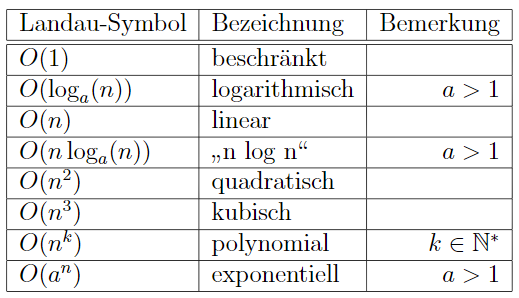
\includegraphics[width=7cm]{landau.PNG} \\

    \bottomrule
\end{tabularx}
\end{table}

\section{Reihen}
\noindent
\textbf{Definitionen}
\begin{table}[H]  
\begin{tabularx}{\textwidth}{X m{16cm}}
    \toprule
    
    & \\

    \bottomrule
    
\end{tabularx}
\end{table}

\noindent 
\textbf{Sätze}
\begin{table}[H]
\begin{tabularx}{\textwidth}{X m{16cm}}
    \toprule

    & \\

    \bottomrule
\end{tabularx}
\end{table}

\noindent
\textbf{Bemerkungen}
\begin{table}[H]
\begin{tabularx}{\textwidth}{X m{16cm}}
    \toprule

    & \\

    \bottomrule
\end{tabularx}
\end{table}

\noindent
\textbf{Beispiele}
\begin{table}[h]
\begin{tabularx}{\textwidth}{X m{16cm}}
    \toprule

    & \\

    \bottomrule
\end{tabularx}
\end{table}
\subsection{Absolute Konvergenz}
\subsection{Das Cauchy-Produkt}


\end{document}